\section*{5. Results Summary}
All three modules and the test bench compiled without errors. The simulated outputs below are read from the waveform in Figure~\ref{fig:wave}; ``Expected'' is the truth table from Section 2.

% 截圖原檔是整個 ModelSim 視窗 (1920x1040)，用 trim/clip 只裁出程式碼區，不改動原圖
% trim = 左 下 右 上 (單位 bp，PNG 無 DPI 資訊時 1 px = 1 bp)

\subsection*{AND Gate}
\begin{figure}[H]
    \centering
    \begin{minipage}[t]{0.48\textwidth}
        \vspace{0pt}
        \centering
        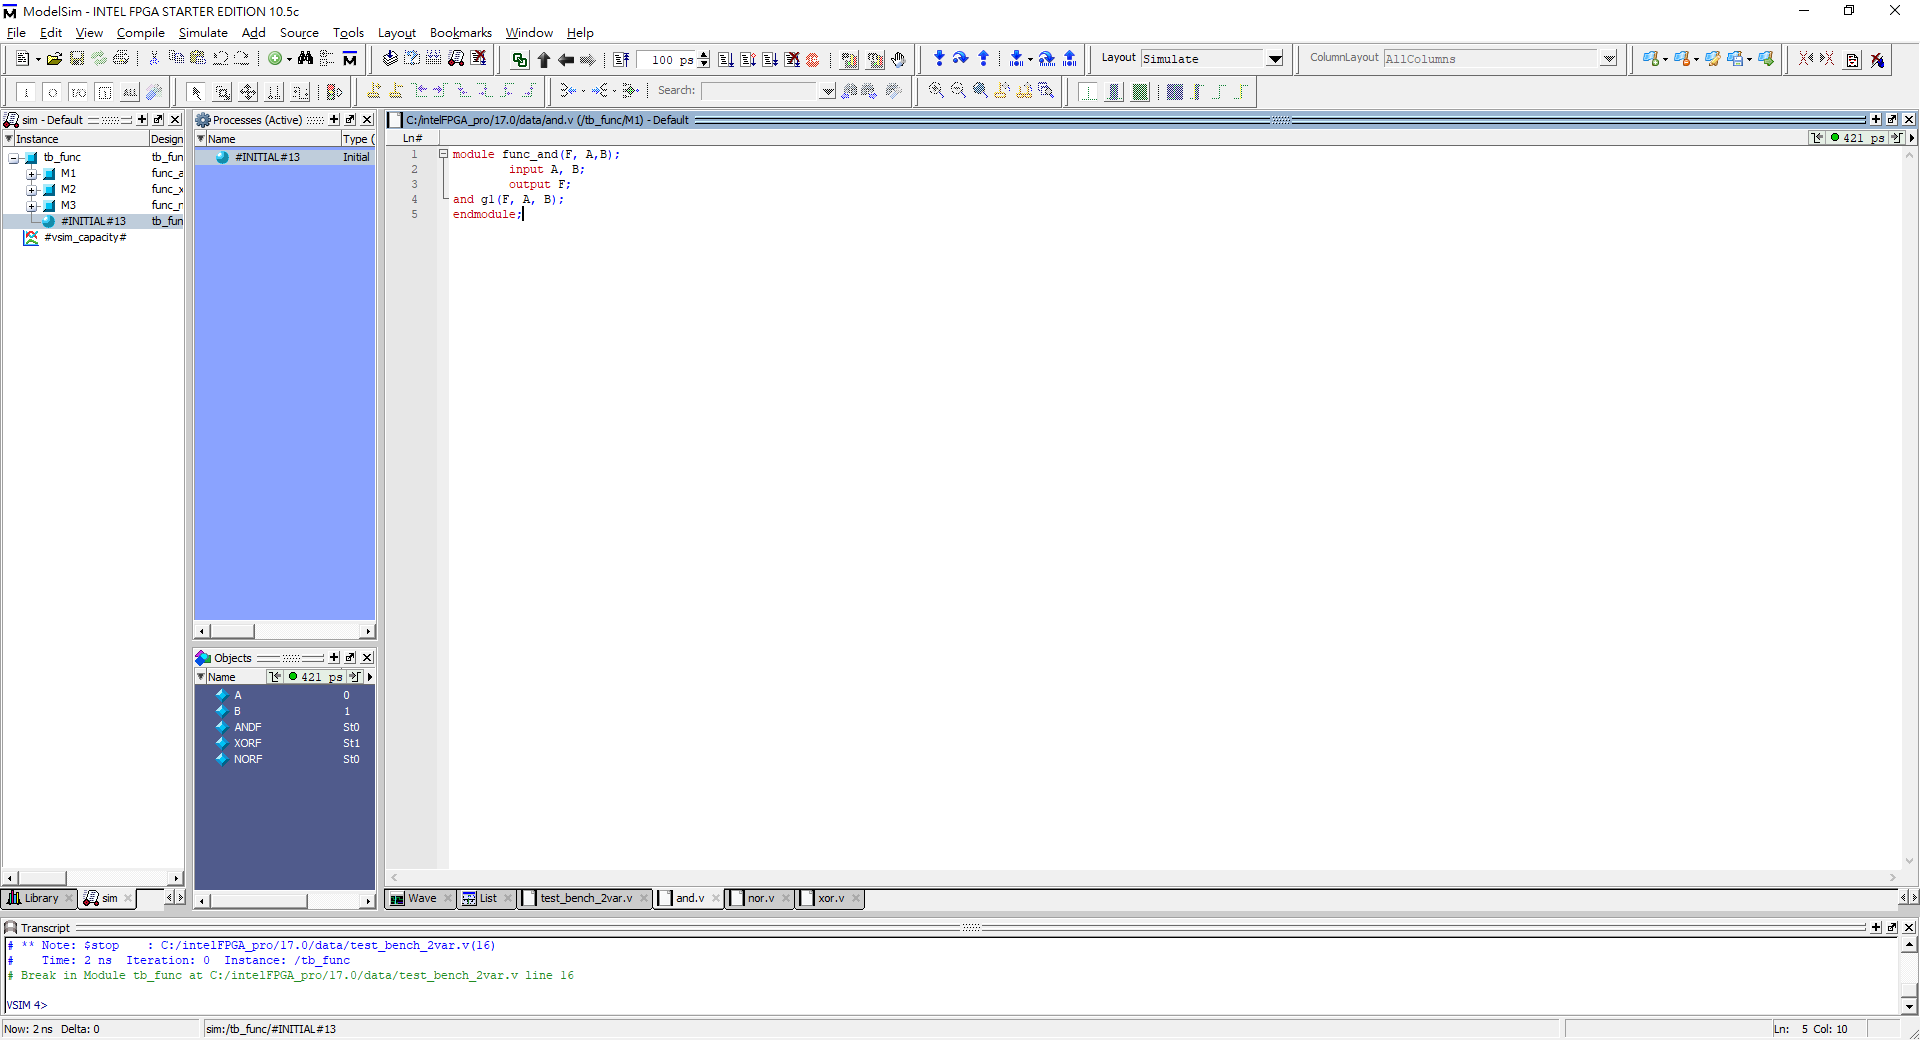
\includegraphics[width=\linewidth, trim=385 815 1160 112, clip]{pic/and.png}
        \captionof{figure}{\texttt{and.v} (module \texttt{func\_and})}
        \label{fig:and}
    \end{minipage}
    \hfill
    \begin{minipage}[t]{0.48\textwidth}
        \vspace{0pt}
        \centering
        \small
        \begin{tabularx}{\linewidth}{c c | >{\centering\arraybackslash}X | >{\centering\arraybackslash}X}
        \toprule
        \textbf{In A} & \textbf{In B} & \textbf{Expected} & \textbf{Simulated} \\
        \midrule
        0 & 0 & 0 & 0 \\
        0 & 1 & 0 & 0 \\
        1 & 0 & 0 & 0 \\
        1 & 1 & 1 & 1 \\
        \bottomrule
        \end{tabularx}
        \captionof{table}{AND gate truth table vs.\ simulation}
        \label{tab:and}
    \end{minipage}
\end{figure}

\subsection*{XOR Gate}
\begin{figure}[H]
    \centering
    \begin{minipage}[t]{0.48\textwidth}
        \vspace{0pt}
        \centering
        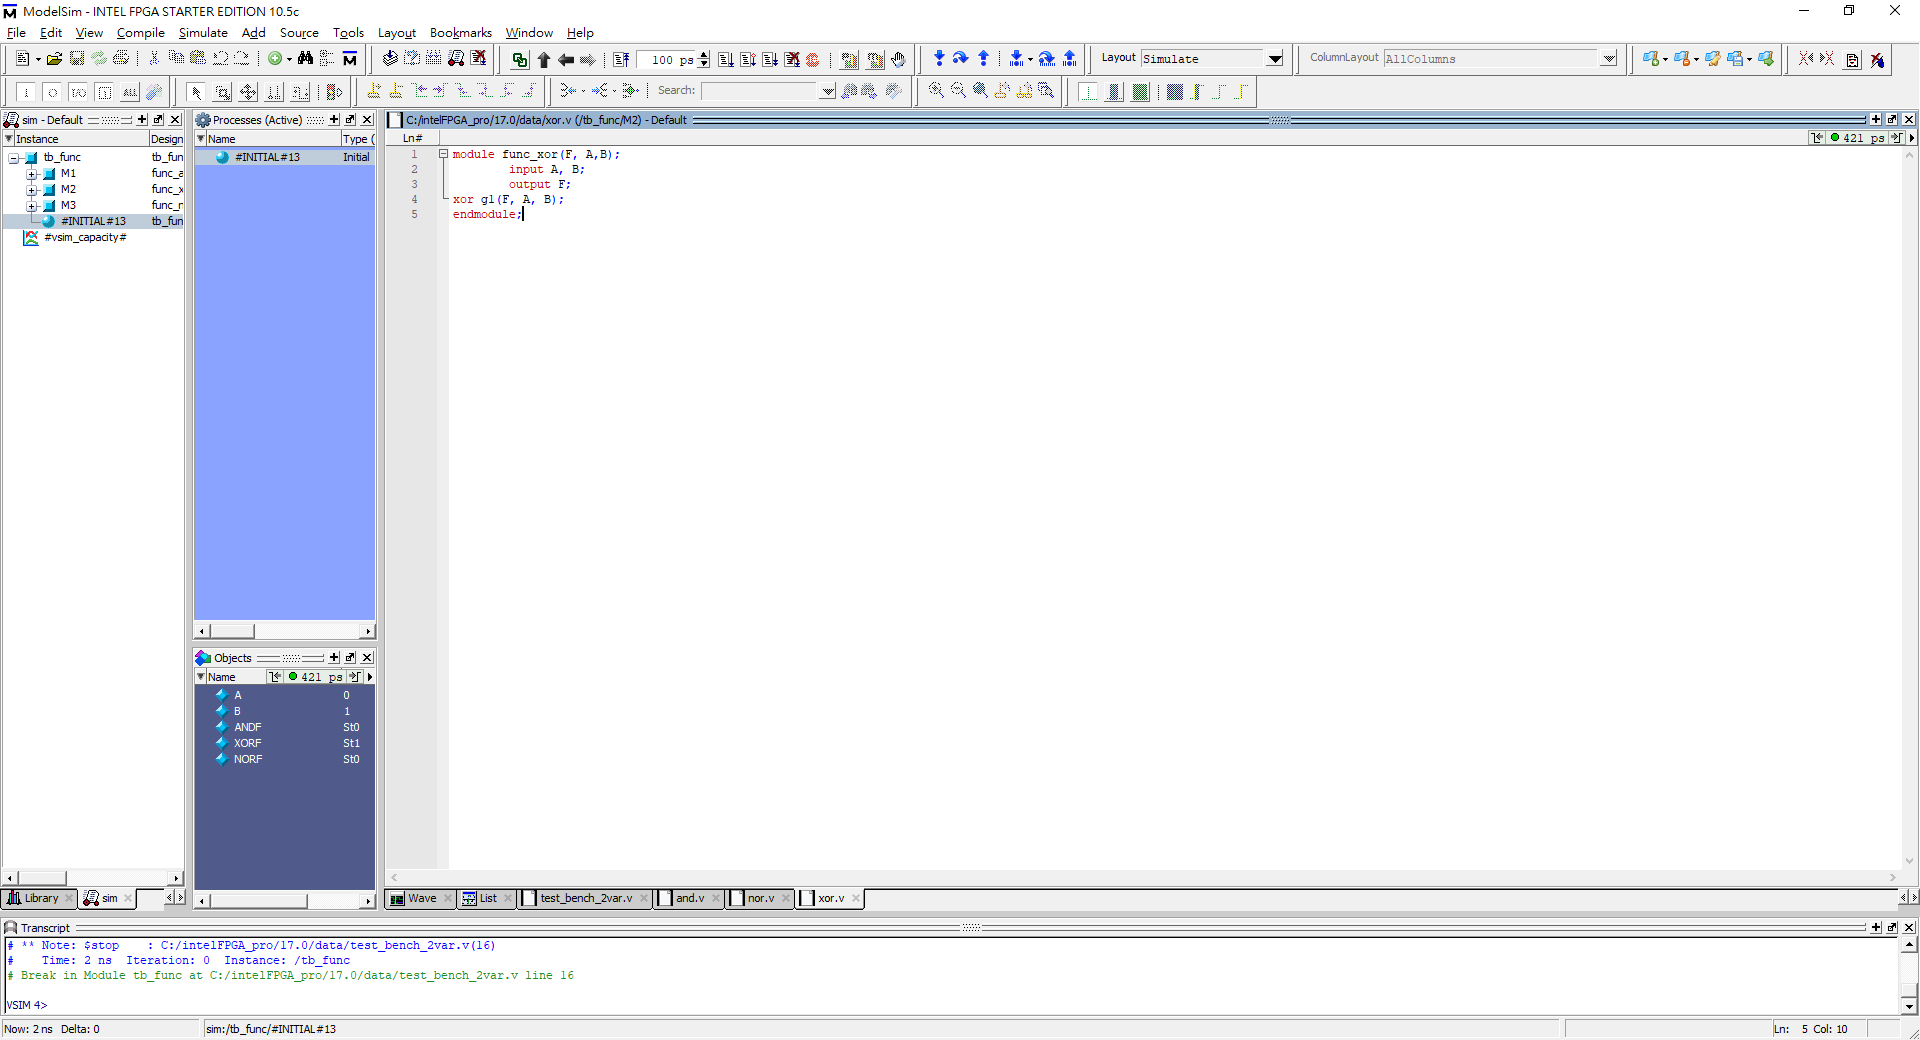
\includegraphics[width=\linewidth, trim=385 815 1160 112, clip]{pic/xor.png}
        \captionof{figure}{\texttt{xor.v} (module \texttt{func\_xor})}
        \label{fig:xor}
    \end{minipage}
    \hfill
    \begin{minipage}[t]{0.48\textwidth}
        \vspace{0pt}
        \centering
        \small
        \begin{tabularx}{\linewidth}{c c | >{\centering\arraybackslash}X | >{\centering\arraybackslash}X}
        \toprule
        \textbf{In A} & \textbf{In B} & \textbf{Expected} & \textbf{Simulated} \\
        \midrule
        0 & 0 & 0 & 0 \\
        0 & 1 & 1 & 1 \\
        1 & 0 & 1 & 1 \\
        1 & 1 & 0 & 0 \\
        \bottomrule
        \end{tabularx}
        \captionof{table}{XOR gate truth table vs.\ simulation}
        \label{tab:xor}
    \end{minipage}
\end{figure}

\subsection*{NOR Gate}
\begin{figure}[H]
    \centering
    \begin{minipage}[t]{0.48\textwidth}
        \vspace{0pt}
        \centering
        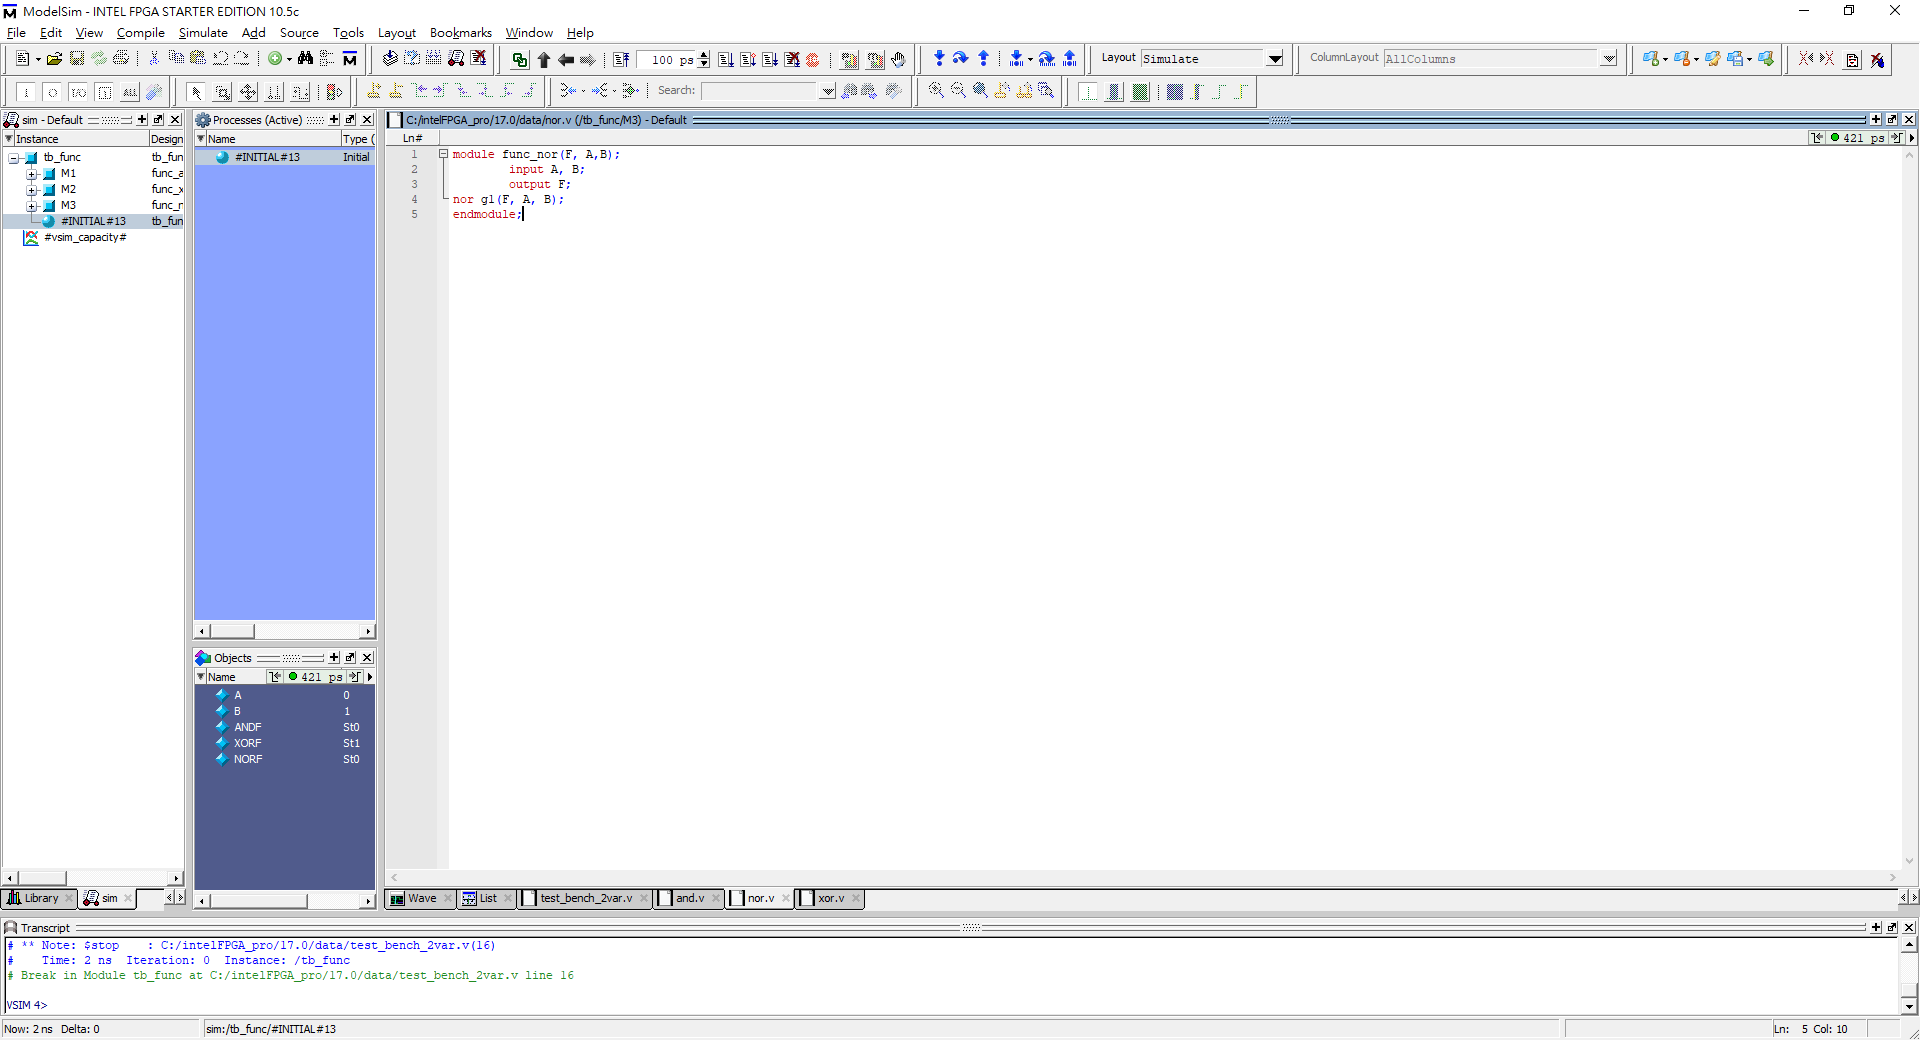
\includegraphics[width=\linewidth, trim=385 815 1160 112, clip]{pic/nor.png}
        \captionof{figure}{\texttt{nor.v} (module \texttt{func\_nor})}
        \label{fig:nor}
    \end{minipage}
    \hfill
    \begin{minipage}[t]{0.48\textwidth}
        \vspace{0pt}
        \centering
        \small
        \begin{tabularx}{\linewidth}{c c | >{\centering\arraybackslash}X | >{\centering\arraybackslash}X}
        \toprule
        \textbf{In A} & \textbf{In B} & \textbf{Expected} & \textbf{Simulated} \\
        \midrule
        0 & 0 & 1 & 1 \\
        0 & 1 & 0 & 0 \\
        1 & 0 & 0 & 0 \\
        1 & 1 & 0 & 0 \\
        \bottomrule
        \end{tabularx}
        \captionof{table}{NOR gate truth table vs.\ simulation}
        \label{tab:nor}
    \end{minipage}
\end{figure}

\subsection*{Test Bench}
The three modules are tested together in one test bench \texttt{tb\_func}: they share the inputs \texttt{A} and \texttt{B}, and drive the outputs \texttt{ANDF}, \texttt{XORF} and \texttt{NORF}.

\begin{figure}[H]
    \centering
    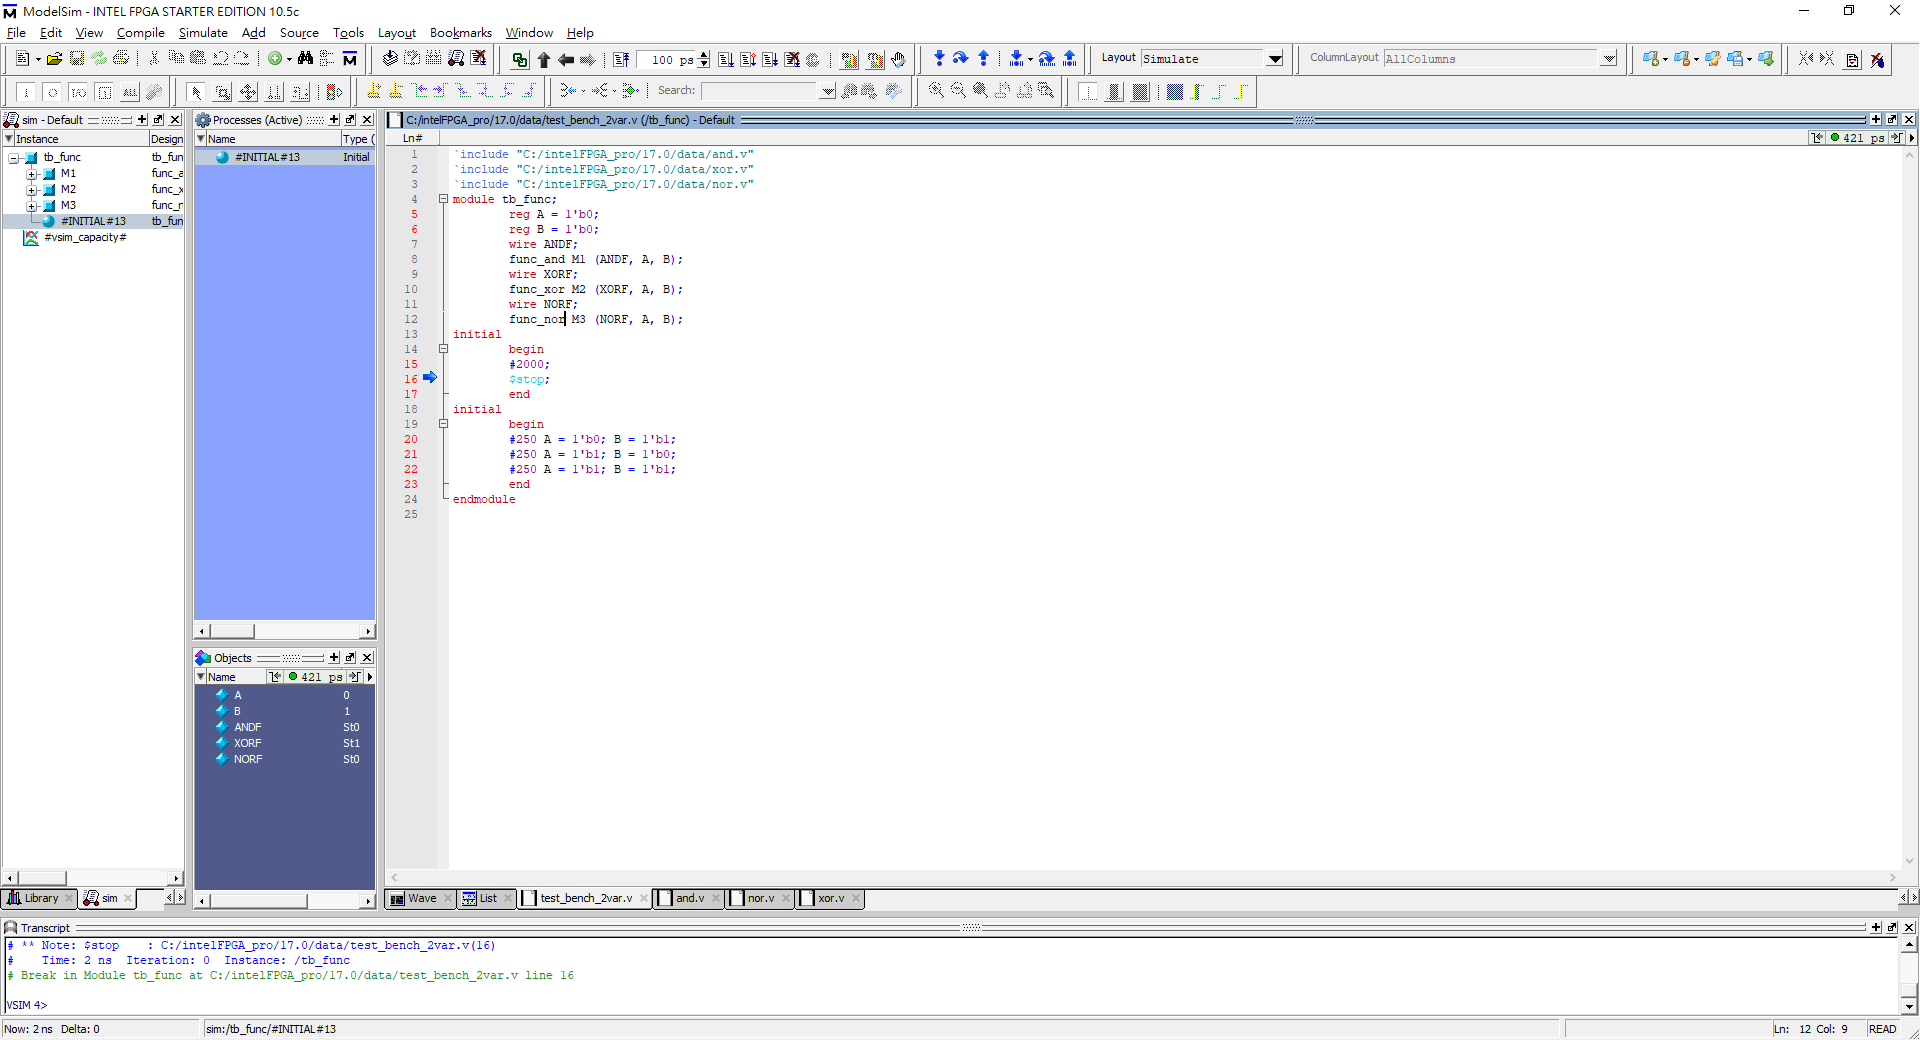
\includegraphics[width=0.6\textwidth, trim=385 532 1120 112, clip]{pic/test.png}
    \captionof{figure}{\texttt{test\_bench\_2var.v} (module \texttt{tb\_func})}
    \label{fig:tb}
\end{figure}

\subsection*{Simulation Waveform}
\begin{table}[H]
\centering
\small
\begin{tabular}{c c c | c c c}
\toprule
\textbf{Time (ps)} & \textbf{A} & \textbf{B} & \textbf{ANDF} & \textbf{XORF} & \textbf{NORF} \\
\midrule
0 -- 250    & 0 & 0 & 0 & 0 & 1 \\
250 -- 500  & 0 & 1 & 0 & 1 & 0 \\
500 -- 750  & 1 & 0 & 0 & 1 & 0 \\
750 -- 2000 & 1 & 1 & 1 & 0 & 0 \\
\bottomrule
\end{tabular}
\captionof{table}{Signal values read from the waveform}
\label{tab:wave}
\end{table}

\begin{figure}[H]
    \centering
    % 上段：訊號名稱與波形；下段：時間軸（中間全黑的空白區裁掉）
    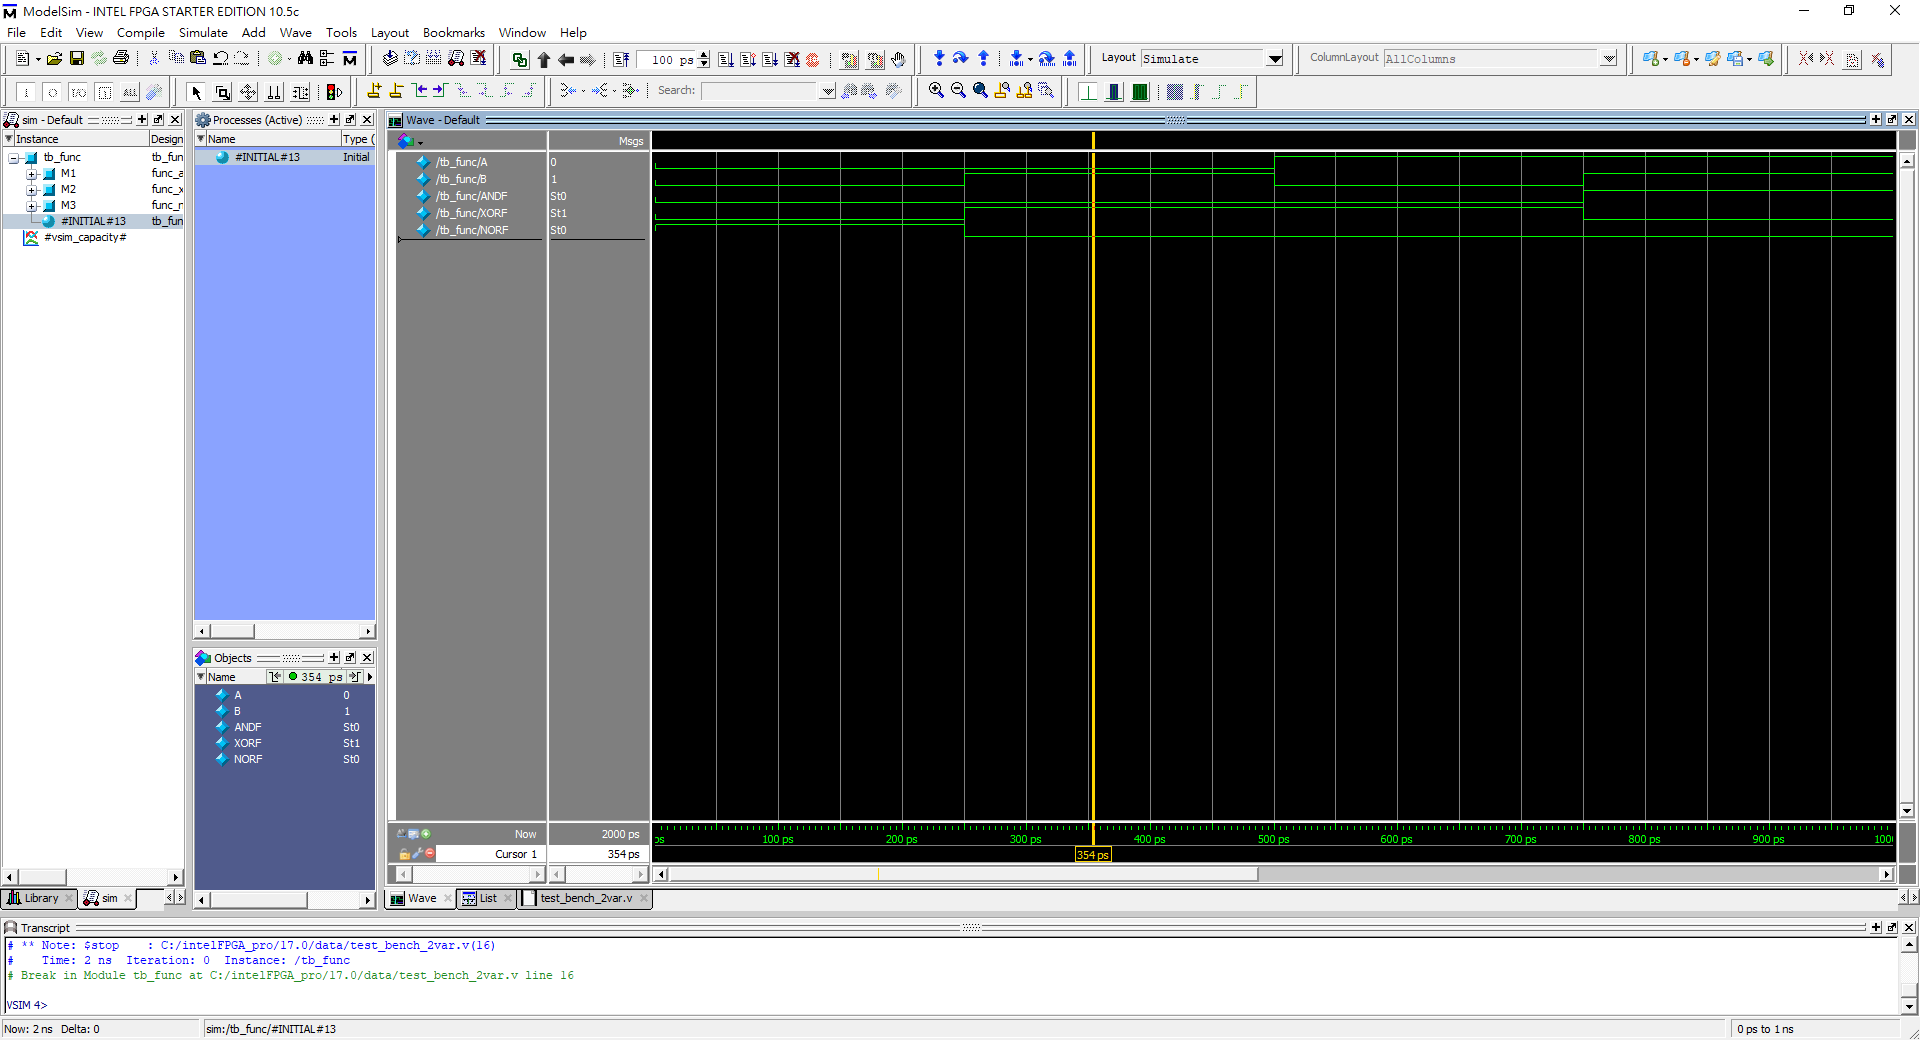
\includegraphics[width=\textwidth, trim=385 790 20 112, clip]{pic/result.png}\\[-1pt]
    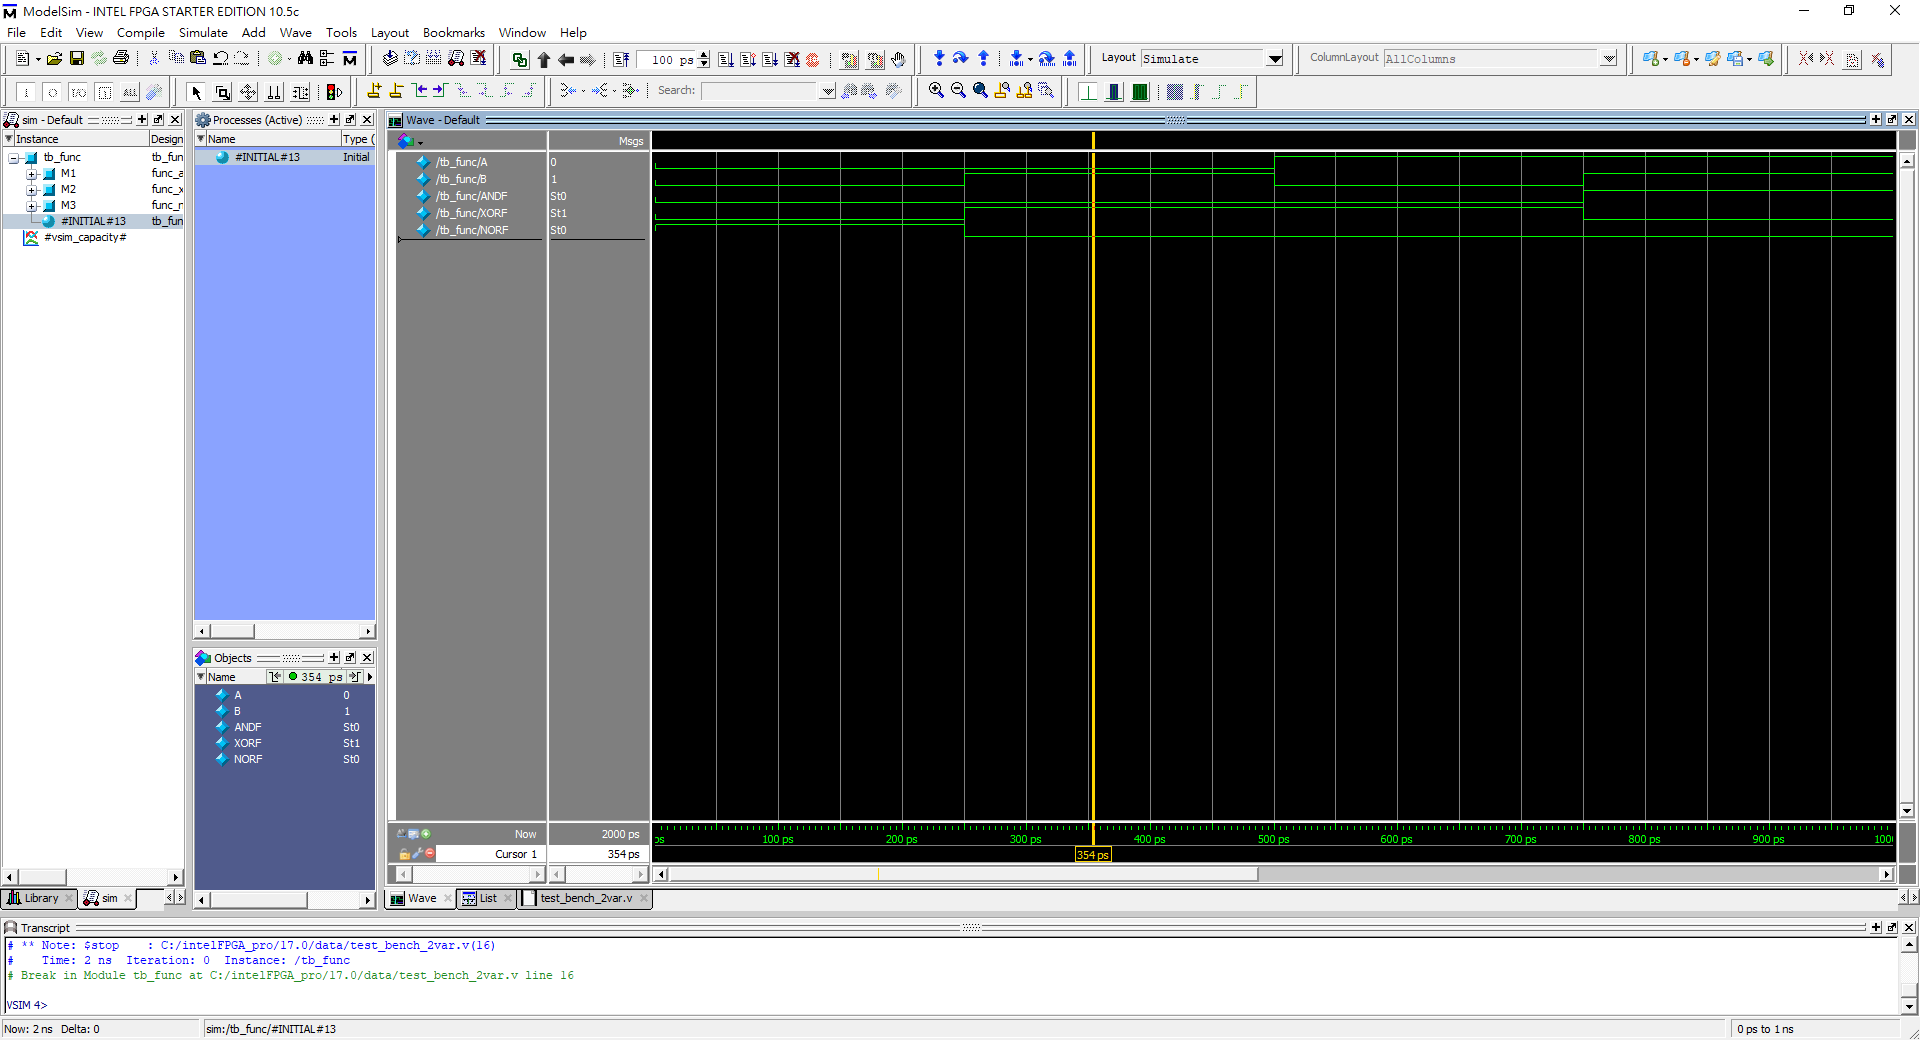
\includegraphics[width=\textwidth, trim=385 175 20 820, clip]{pic/result.png}
    \captionof{figure}{Simulation waveform (cursor at 354 ps: $A=0$, $B=1$, ANDF $=0$, XORF $=1$, NORF $=0$)}
    \label{fig:wave}
\end{figure}

The simulated outputs of all three gates match their truth tables for every input combination.
